% !TeX TXS-program:compile = txs:///pdflatex/[--shell-escape]
\documentclass[a4paper,12pt,oneside]{report}

% set font to Times New Roman
\usepackage{fontspec}
\setmainfont{Times New Roman}

% setup images folder
\usepackage{graphicx}
\graphicspath{{images/}}

% configure the geometry of the paper
\usepackage[
	a4paper,
	showframe=false,
	top=3cm,
	bottom=3cm,
	left=3cm,
	right=3.5cm,
	bindingoffset=6mm
]{geometry}
\setlength{\headheight}{15pt}

% add spacing environment
\usepackage{setspace}

% figure placement package
\usepackage{float}

% set linespacing to 1.5
\renewcommand{\baselinestretch}{1.5}

% set linespacing in footnotes to 1.0
\let\origfootnote\footnote
\renewcommand{\footnote}[1]{
	\begingroup
	\renewcommand{\baselinestretch}{1.0}
   	\origfootnote{#1}
   	\endgroup
}

% remove indentation for footnotes
\usepackage[hang,flushmargin]{footmisc}

% allow filling cells in tables
\usepackage[table]{xcolor}

% allow specifying row heights in tables
\usepackage{stackengine}
\newcommand\xrowht[2][0]{\addstackgap[.5\dimexpr#2\relax]{\vphantom{#1}}}

% center caption in figures and listings
\usepackage[justification=centering]{caption}
% \captionsetup[listing]{position=top}
\captionsetup{labelfont=bf}

% setup minted package for listings
\usepackage[friendly]{minted}

% add enumeration package for lists
\usepackage{enumitem}

\usepackage{etoolbox}
\apptocmd{\sloppy}{\hbadness 10000\relax}{}{}

% setup glossaries (acronyms)
% \usepackage[
% 	toc,
% 	acronym,
% 	xindy={glsnumbers=false},
% 	nonumberlist,
% 	nopostdot,
% 	nogroupskip
% ]{glossaries}
% \makeglossaries

\usepackage[pdfborder={0 0 0}]{hyperref}
\usepackage{cleveref}

% add "List of Figures" and "List of Listings" to ToC
\usepackage[nottoc]{tocbibind}

% setup page header
\usepackage{fancyhdr}
\pagestyle{fancy}
\fancyhf{}
\fancyhead[L]{\bfseries\nouppercase\rightmark}
\fancyhead[R]{\bfseries\thepage}

% setup bibliography
% \usepackage[style=apa,url=true,sorting=nty,backend=biber]{biblatex}
% \usepackage{csquotes}
% \addbibresource{references.bib}
\renewcommand{\UrlFont}{\small\tt}

\title{The environmental impact of programming language choice}
\author{Paula Dettmann}
\date{Spring 2022}

\makeatletter
\let\thetitle\@title
\let\theauthor\@author
\let\thedate\@date
\makeatother

\begin{document}

\newgeometry{
	top=3cm,
	bottom=3cm,
	left=2.5cm,
	right=3cm,
	bindingoffset=6mm
}

\begin{titlepage}
	\begin{center}
		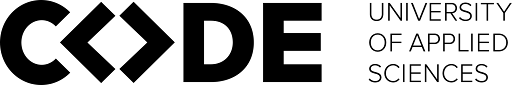
\includegraphics[width=0.5\textwidth,scale=0.55]{university-logo}

		\vspace*{0.8cm}

		\textbf{Software Engineering}\\
		\textbf{Bachelor Thesis}

		\vfill

		\textbf{\large\thetitle}
	\end{center}

	\vfill

	\noindent\hspace{1mm}\makebox[2in]{\rule{2in}{0.4mm}}
	\vspace{5mm}

	\begin{spacing}{1.1}
		\noindent
		\setlength{\tabcolsep}{20pt}
		\begin{tabular}{@{}ll}
		\textbf{Name:} & \theauthor \\
        \textbf{Address:} & Paulsborner Straße 91, 10709 Berlin \\
        \textbf{E-mail:} & paula.dettmann@code.berlin\\
        \\
        \textbf{Date of Submission:} & 03.06.2022\\
        \\
        \textbf{Student ID} & 19.03.024 \\
		\textbf{Semester:} & Spring 2022\\
		\\
		\textbf{First Assessor:} & Prof. Dr. Adam Roe\\
		\textbf{Second Assessor:} & Dipl-inf. Fabio Fracassi\\
		\end{tabular}
	\end{spacing}
\end{titlepage}


\newgeometry{
	top=3cm,
	bottom=3cm,
	left=3cm,
	right=3.5cm,
	bindingoffset=6mm
}

\pagenumbering{roman}

% \input{dedication}
% \chapter*{Acknowledgements}

I would like to express my appreciation to to my supervisors Prof. Dr. Adam Roe and Dipl-inf. Fabio Fracassi for their invaluable guidance and feedback.
I am also grateful to my family and partner, for their editing help and moral support.

Climate change is a problem that humanity needs to combat.
Software engineers can contribute to the fight against global warming by writing energy-efficient software.
This thesis explores which environmental impact the choice of programming language can have.
By writing image processing programs in C++ and Python and benchmarking them using different configurations of software and
hardware, we found that while a programming language in isolation can affect the energy efficiency of a program,
writing software does not happen in isolation.
Therefore, every configuration of software and hardware affects the energy efficiency of a program.
If one part is not optimised, it can increase the total runtime of the program by a significant amount.
Therefore, we can conclude that the choice of programming language can only impact the runtime if all other factors of the program's configuration are optimised.


\tableofcontents
\listoffigures
\listoflistings

% \input{acronyms}
% \setlist[description]{leftmargin=!, labelwidth=5em}
% \printglossary[type=\acronymtype,title={List of Abbreviations}]
\setlist[description]{style=standard}
\newpage

\pagenumbering{arabic}

\chapter{Introduction}
\setcounter{page}{1}

This thesis is about the environmental impact of the choice of programming language. Every operation on a computer takes up energy. Extrapolating the usage of a single computer to a global operation, the required energy of single operations becomes significant. Therefore, software engineers need to optimise their programs to take up the least amount of energy possible. This thesis researches which part the choice of programming language plays in energy efficiency.
Other research has been done on the most efficient programming languages, testing several algorithms in different languages and determining the most efficient ones, which proved to be C, Rust and C++. We set out to experiment with a more realistic program, with disk I/O (disk input and output) and other operations as well as an algorithm. We tested the same program in Python and C++ and benchmarked the runtime of each operation in the program.
According to a study at Queens University in Ontario, Canada, programmers have limited knowledge about energy efficiency, lack knowledge about the best practice to reduce the energy consumption of software, and are often unsure about how software consumes energy \cite{programmers}.
Therefore, our research is essential to perhaps ultimately serve as a recommendation on how to reduce energy usage by making a programming language choice. At the very least, to make developers think about the environmental impact of their software by putting forth observations on its environmental impact.
This research hypothesises an environmental impact on the choice of programming language. This hypothesis will be proved or disproved through a series of experiments where we benchmark the same image processing program in C++ and Python in different hardware and software configurations. We aim to observe which language runs fastest.
First, we aim to give a general introduction to green computing and the programming languages we will be exploring. A small part of the paper will report previous research on the energy efficiency of programming languages and how we utilised this research in this thesis. Another chapter will illustrate the research hypothesis and explain how it can be proved or disproved. The next chapter will cover the research methods, including the code and profilers. Then we will display the results of the experiments that were done and discuss the results in the following chapter. Lastly, there will be a conclusion and bibliography.

\chapter{Green Computing}

Power electronics are an ever-increasing part of the energy sector. Therefore, a way to conserve energy to aid in the fight against global warming has emerged: green computing.
Green computing is the environmentally responsible and eco-friendly use of computers and their resources \cite{Salama20}. Green computing first started when the US Environmental Protection Agency launched Energy Star in 1992, a label that stands for energy efficiency in monitors, climate control equipment, and other technologies \cite{ENERGYSTAR}.
Later, Swedish TCO development launched the TCO certified program to promote low magnetic and electrical emissions from CRT-based computer displays, energy consumption, ergonomics, and the use of hazardous materials in construction. It is still active, 30 years later, constantly updating its criteria according to technological improvements \cite{TCOCertified}.
There are several aspects to green computing. First of all, the software itself, meaning algorithm optimisation and programming language choice. Choice of deployments can also play a big part. For example, it matters where servers that developers choose to run their code on are located because colder climates and locations close to a water source save energy needed for cooling. Additionally, it is important what kind of energy is used, namely fossil or renewable energy. Another aspect is the make of the servers and physical tools that a developer uses. Some servers are more efficient than others, and some are made with recycled or eco-friendly materials.
The aspect that we would like to focus on in this paper is green software.

\section{Quantifying environmental impact}
One standard to measure environmental impact is using the Greenhouse Gas Protocol (GHG). The GHG is a “comprehensive global standardised framework to measure and manage greenhouse gas (GHG) emissions from private and public sector operations, value chains and mitigation actions.” \cite{GHGProtocol} Companies like “AMD, Apple, Facebook, Google, Huawei, Intel, and Microsoft publish annual sustainability reports using the GHG Protocol.”\cite[p.855]{9407142}  The GHG categorises emissions into three scopes. “Scope one emissions come from fuel combustion (e.g., diesel, natural gas, and gasoline), refrigerants in offices and data centres, transportation, and the use of chemicals and gases in semiconductor manufacturing.” \cite[p.856]{9407142}. Scope two emissions “come from purchased energy and heat powering semiconductor fabs, offices, and data-centre operation.” \cite[p.856]{9407142} These emissions are relevant to software engineers. Scope three “emissions come from all other activities, including the full upstream and downstream supply chain. They often comprise employee business travel, commuting, logistics, and capital goods”. \cite[p.856]{9407142}
The scope that we can influence with software is scope two. Using AI as an example, a paper by U. Gupta (et al.) called Chasing Carbon: The Elusive Environmental Footprint of Computing describes that “algorithmic optimisations for scale-down systems will drastically cut emissions.” \cite[p.863]{9407142}
We can reason that there is a direct correlation between the speed of a program and the amount of data centres. When a program is less optimised, it runs for a more extended period, occupying data centres for a longer time. Therefore, the demand for data centres rises, causing companies to build more data centres, a CO2 intensive process. According to a paper by Md Abu Bakar Siddik, Arman Shehabi and Landon Marston, “approximately 0.5\% of total US greenhouse gas emissions are attributed to data centres” \cite{Siddik_2021}.

\chapter{Programming Languages}

Programming languages are different levels of binary abstraction, the ones and zeroes that make up the computer's language. Commands to the computer are written in a particular language and then compiled into binary.
These compilers are different for each language. Each language also has a different garbage collection form, redundant data handling, and other specifics. Therefore, each language has certain specialities and operates at different speeds.
We make a distinction between high level and low-level languages. High-level languages compile automatically at runtime and have built-in garbage collection. Some low-level languages require developers to handle garbage collection themselves and compile their code into an executable file before running it.
That makes lower-level languages more customisable and, as a result, often faster.
Therefore, we consider low-level languages like C++ and Rust to be faster for most use-cases, and higher-level languages like Python and JavaScript are considered slower.
In this thesis, C++, a low-level language and Python, a high-level language, are pitted against each other to explore what difference the choice of language makes on the same application in terms of speed and energy efficiency.

\section{C++}
C++ is based on the traditional C language. We consider C++ a low-level language because it lacks automatic memory management. Many different compilers are available for C++, making it a portable language. "C++ compiles directly to a machine's native code, allowing it to be one of the fastest languages in the world if optimised" \cite{C++}.
For the research in this thesis an Apple MacBook computer was used. The Operating System (OS) is macOS Monterey, which ships with the C++ compiler clang, as seen in figure 3.1. “The Clang project provides a language front-end and tooling infrastructure for languages in the C language family (C, C++, Objective C/C++, OpenCL, CUDA, and RenderScript) for the LLVM project” \cite{clang}. Clang is also used in production to build software like Chrome or Firefox. The clang compiler is incorporated into the macOS native Xcode IDE (integrated development environment), which was used for the research in this thesis.

\begin{figure}[htbp]
	\centering
	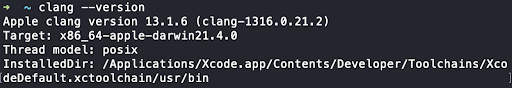
\includegraphics[scale=0.72]{clang.png}
	\caption{clang version on MacBook Pro}
	\label{figure:clang}
\end{figure}

\section{Python}
Python is an open-source, interpreted, object-oriented programming language. "It incorporates modules, exceptions, dynamic typing, very high-level dynamic data types, and classes." It runs on many operating systems like macOS, Windows and Linux.
The language comes with a sizeable standard library for many different purposes. For example, Python is often used for experimenting and logging, string processing and internet protocols like HTTP. Besides the standard library, there is also a wide variety of third-party extensions available \cite{python}.

\chapter{Previous Research}
The choice of programming languages was based on a study that ranked different programming languages by their energy efficiency. The study pitted ten programming languages against each other, using “rigorous and strict solutions to 10 well-defined programming problems, expressed in (up to) 27 programming languages, from the well known Computer Language Benchmark Game repository.” \cite[abstract]{PEREIRA2021102609} Results of the study showed that C++, C and Rust were the most energy-efficient languages and time efficient, with Pascal and Go scoring higher on memory efficiency, as seen in figure 4.1. Python consistently scored in second to last place for energy and time efficiency and in 12th place (out of 27 languages) for memory efficiency.
C++ was chosen based on the libraries available for the chosen aim of the program and because it was one of the best performing languages in this study.
Python was chosen because it was one of the three worst-performing languages in the study.

\begin{figure}[htbp]
	\centering
	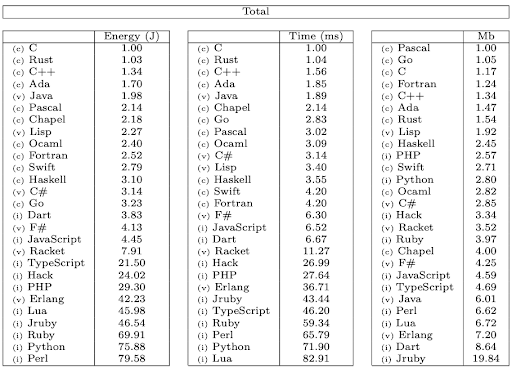
\includegraphics[scale=0.70]{previous-research-languages.png}
	\caption{Normalised global results for Energy, Time, and Memory \cite[p.16]{PEREIRA2021102609}}
	\label{figure:previous-research-languages}
\end{figure}

\chapter{Research Hypothesis}
This thesis’s research hypothesis was that there is an environmental impact based on the choice of programming language for a particular application.
The hypothesis would be proved correct if one programming language performed measurably better than another. This was measured by benchmarking the same image processing application in two languages. Observations were made on the speed of the different parts of the application; the image blurring algorithm, the disk input, the disk output and other operations. The overall energy consumption of the program could also be measured.
Testing the hypothesis was done according to the scientific method. This means performing an experiment and collecting data in a reproducible manner. The experiment was controlled, meaning that all variables besides the programming language were the same, as far as that was possible. By this method, it could be ensured that the result of the experiment pertained to the programming language and no other factors such as the library, OS, IDE or profiler.
A weakness of this study might be that it is not always possible to eliminate all variables because of compatibility issues with the programming languages. For example, a profiler that works for C++ will not work in the same capacity for Python code and, therefore, might produce slightly different results.
The results of this research could guide environmentally conscious developers on how to reduce their environmental impact for an image processing project.

\chapter{Methods}
In order to prove the hypothesis, we wrote a small program to blur images. The kind of program was not important, but it was necessary for it to take a significant amount of time and make a measurable impact on the CPU.
We benchmarked the program using profilers. The profiler data shows where delays in the code are located and which language is faster at executing the same procedure. This information allows us to conclude which language, for the purpose of image processing in the form of a Gaussian blur, is more efficient and therefore more environmentally friendly.

\section{Hardware}
Most of the experiments were performed on an Apple MacBook Pro with a 1.4 GHz Quad-Core Intel Core i5 processor. The computer had 16 GB of RAM and 251 GB of flash storage. It was running version 12.3.1 of the MacOS Monterey operating system.

\section{Profilers}
A profiler is a benchmarking tool. It measures the runtime of a program, and other statistics, depending on the profiler. To benchmark our Python program on macOS, we used a combination of xctrace and cPython. For the C++ code on macOS, we exclusively used xctrace.

\subsection{\textit{time}}
At first, we used the macOS \textit{time} command to measure the runtime of the Python program, as seen in figure 6.1.

\begin{figure}[htbp]
	\centering
	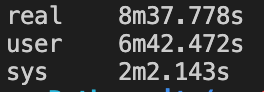
\includegraphics[scale=0.72]{time.png}
	\caption{An example of the \textit{time} command}
	\label{figure:time}
\end{figure}

\textit{time} is a macOS shell keyword that measures the total time spent running the program. The user row shows the time spent in the CPU in user mode, meaning “it does not have direct access to hardware or reference memory and must rely on APIs of the system for delegation. This is how most code runs on your system, and due to its isolation, crashes are always recoverable” \cite{time}. sys stands for system mode or kernel mode. Kernel mode is “when code being executed has unrestricted access to the system hardware” \cite{time}. The first row, called real, is the total time spent in the two modes.

\subsection{XCode Instruments}
In order to keep the research controlled, we decided to use the same profiler for both programs; Xcode instruments. Xcode is Apple’s IDE and contains Instruments amongst other developer tools. “The Instruments app, which is included with Xcode, gathers data from your running app and presents it in a graphical timeline. With Instruments, we can gather data about performance areas such as our app’s memory usage, disk activity, network activity, and graphics operations” \cite{instruments}. The command-line tool for Instruments is called xctrace, and it is used to record, import, export and symbolicate Instruments .trace files. These .trace files can then be opened in the Instruments app and analysed with the graphical user interface. We mostly used the CPU Counter template. It allowed us to track how much time was spent on each part of the program; the algorithm, disk input, disk output and retrieving file names.

\subsection{cProfile}
cProfile is a profiler that is included in the Python standard library. It is a C extension with a reasonable overhead which makes it suitable for profiling long-running programs. It was based on lsprof and contributed by Brett Rosen and Ted Czotter \cite{cprofile}. cProfile measures the total time the program runs, the number of function calls, and the runtime and function calls of each individual function. The measured statistics can be displayed in the command-line interface or a text file.

\section{Energy benchmarking}
We can measure the energy used by the programs using the Intel® Power Gadget. It is a software-based power usage monitoring tool enabled for Intel® Core™ processors. It is supported on Windows and macOS and includes an application, driver, and libraries to monitor and estimate real-time processor package power information in watts using the energy counters in the processor \cite{powergadget}. The command-line tool PowerLog allows us to measure the energy usage of a program and write it to a log file. Specifically, the log file will include the elapsed time, package power limit, processor frequency, GT (Energy of the processor graphics) frequency, processor temperature, and average and cumulative power of the processor.

\section{Code}
We are experimenting with the same algorithm in both languages: Gaussian Blur. In image processing, a Gaussian blur is a result of blurring an image by a two-dimensional Gaussian function which was named after mathematician and scientist Carl Friedrich Gauss. Applying the algorithm to the image causes a blurring effect on the image, the intensity of the blur effect depending on variables like the kernel and standard deviation. We made sure to write the code for the two languages to execute as similar as possible.

\subsection{Python}

\begin{listing}[!ht]
\begin{minted}[xleftmargin=20pt, linenos]{python}
#!/usr/bin/env python

import cv2 as cv
import os
import cProfile

pr = cProfile.Profile()
pr.enable()

img_names = os.listdir("/Volumes/RAMDisk/raw")

for name in img_names:
  path = "/Volumes/RAMDisk/raw/{}".format(name)

  if ".DS_Store" in path:4
    continue

  img = cv.imread(path)
  blur = cv.blur(img,(5,5))

  cv.imwrite("/Volumes/RAMDisk/python_blurred/blurred_" + name, blur)

pr.disable()
pr.print_stats()
\end{minted}
\caption{The Python program}
\label{listing:python}
\end{listing}

Looking at listing 1, os is a module that provides a portable way of using operating system dependent functionality \cite{os}. It is used in line 10 to list all image names in the raw images directory. In line 12, a for loop is used to iterate through that list of names, therefore every picture can be blurred, one at a time. Every picture first is “read” in line 18, after determining the path in line 13 and dismissing a possible macOS bug in case the file “.DS\_Store” exists in the directory in lines 15 and 16. In line 19, the Gaussian blur filter is applied to the image using the OpenCV function with parameters of the image variable and Gaussian kernel size. Line 21 shows the blurred image being written to the disk.
In listing 1, we can also see the profiler cProfile being used. It is imported in line 5 and initialised in line 7. Line 8 enables the profiler and line 23 disables it so it is wrapped around the code we want to profile. In line 24 the collected statistics are printed to the console or a file.

\subsection{C++}

\begin{listing}[!ht]
\begin{minted}[xleftmargin=20pt, linenos]{c++}
#include <opencv2/opencv.hpp>
#include <iostream>
#include <string>
#include <filesystem>
#include <vector>

using namespace cv;
using namespace std;

namespace fs = std::__fs::filesystem;
\end{minted}
\caption{The C++ program requirements}
\label{listing:c++requirements}
\end{listing}

Listing 2 shows the beginning of the C++ code. First, we import the OpenCV and C++ standard libraries and assign the namespaces.

\begin{listing}[ht]
\begin{minted}[xleftmargin=20pt, linenos]{c++}
int main(int argc, char* argv[])
{
  if (argc < 3) {
    cout << "Usage: ./green_apple_blur <input_path> <output_path>" << endl;
    return 1;
  }

  string base_path = argv[1];
  string ds = ".DS_Store";

  for (const auto & file : std::__fs::filesystem::directory_iterator(base_path))
  {
    fs::path path = file.path();
    string filename = path.filename().string();

    if (find(path.begin(),path.end(),ds)!=path.end())
      {
        continue;
      }

\end{minted}
\caption{Reading the image file}
\label{listing:c++-read}
\end{listing}

In listing 3, the path to the images is added as a parameter to the main function when the program is run in line 1. To prevent a bug we ignore the file “.DS\_Store” in the path in line 16.

\begin{listing}[ht]
\begin{minted}[xleftmargin=20pt, linenos]{c++}

    // Read the image file
    Mat image = imread(path);

    // Check for failure
    if (image.empty())
      {
        cout << "Could not open or find the image" << endl;
        cin.get(); //wait for any key press
        return -1;
      }

    //Blur the image with 5x5 Gaussian kernel
    Mat image_blurred;
    GaussianBlur(image, image_blurred, Size(5, 5), 0);

    string writePath = argv[2];

    string blur_path = writePath + "/blurred_" + filename;
    bool isSuccess = imwrite(blur_path, image_blurred); //write the image to a file as JPEG

    if (isSuccess == false)
      {
        cout << "Failed to save the image" << endl;
        cin.get(); //wait for a key press
        return -1;
      }
    }

    return 0;
}
\end{minted}
\caption{Processing and writing the image file to the disk}
\label{listing:c++-write}
\end{listing}

In line 2 of listing 4, we read the image file with the OpenCV imread function. In line 14 we blur the image with the GaussianBlur filter function from OpenCV \cite{gaussianblur}. Size (5, 5) is the Gaussian kernel size, it should be an odd number. The last zero controls the sigma value which is the standard deviation in the X direction and the Y direction of the Gaussian distribution. It will be calculated based on the size of the kernel \cite{gaussianblurtutorial}. In line 19 we save the image to the path specified in the parameter and check whether that succeeded. At the end, we return 0 to terminate the function successfully.

\chapter{Results}
In order to discern whether the choice of programming language has an environmental impact, experiments were executed, each time changing a different aspect of the experiment to see if there is a significant difference between the performance of the languages. Most experiments used the programs to blur 78 high definition images.

\section{C++ and Python with OpenCV }
The first experiment was to run our programs with the chosen profiler of xctrace and cProfile to determine the runtime of each function in the program, blurring 78 images in total. Each benchmark was run five times and then the average was calculated. We see the result of these experiments in figure 7.1.

\begin{figure}[H]
	\centering
	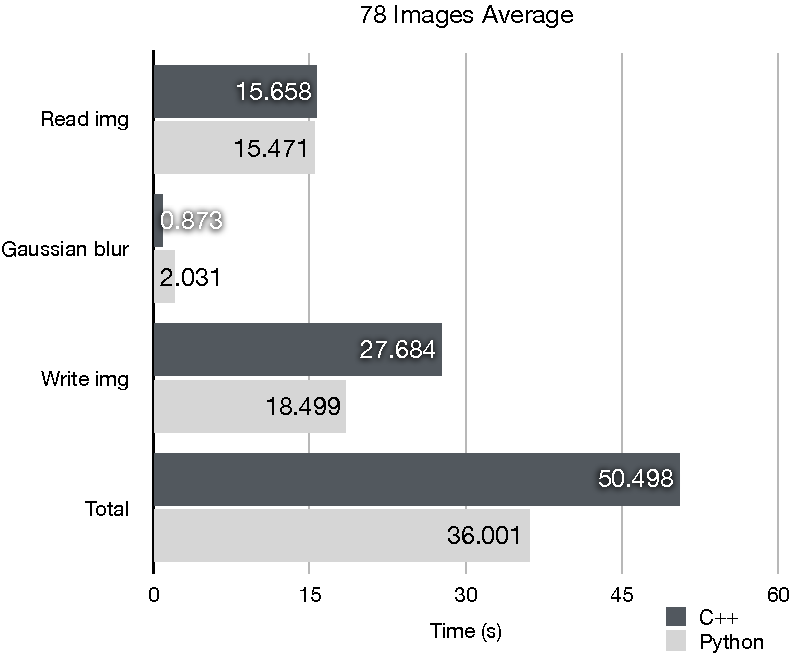
\includegraphics[scale=0.72]{average-without-script.pdf}
	\caption{The average of 5 runs for each language}
	\label{figure:average-78img}
\end{figure}

These results were highly uncharacteristic. Based on previous research, it was expected that C++ would be faster than Python, not slower. Most of the delay for C++ seemed to come from writing the blurred image to the disk, as seen in the write-img-bars in figure 7.1.

\section{Saving to BMP instead of JPEG}
One approach to solving the significant delay of C++ when writing images to the disk was to change the file type of the image for both languages. The default settings of the OpenCV package saved the image to whichever file type the image had initially been; in this case, that was JPEG (Joint Photographic Experts Group). Changing the file extension from JPEG to BMP (bitmap image file) would change the image file type on saving the image. Strangely, as seen in figure 7.2, this warped the data in such a way that reading the image now took longer for C++ and writing the image was quite a bit faster. It is assumed that this might be attributed to the library version, but further research is needed to confirm this.

\begin{figure}[H]
	\centering
	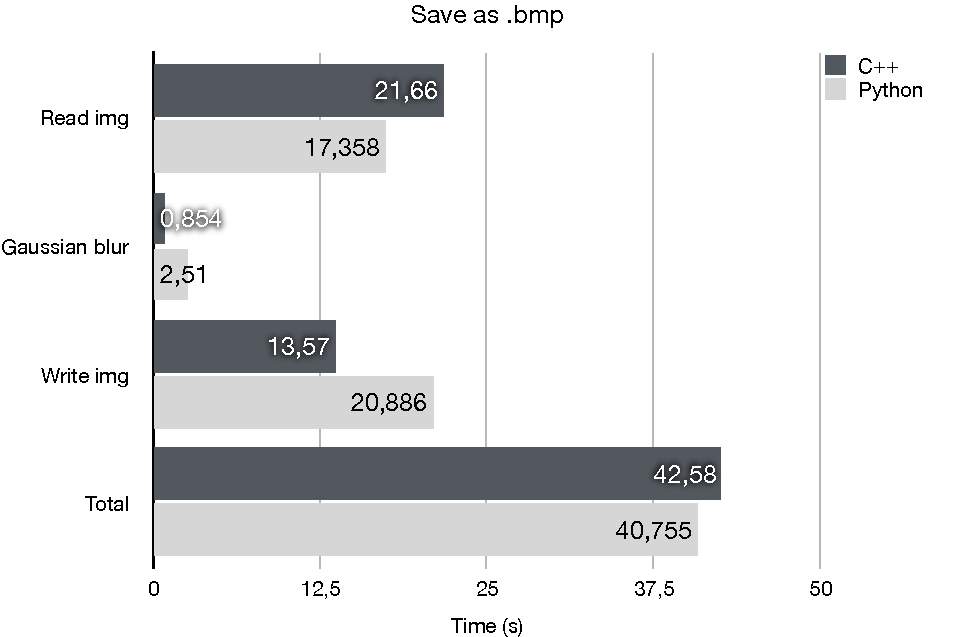
\includegraphics[scale=0.72]{bmp.pdf}
	\caption{Saving the image as a BMP file}
	\label{figure:bmp}
\end{figure}

\section{Using a script to benchmark}
The following experiment was to benchmark the programs using a script. A script is a sequence of instructions that are carried out subsequently by a computer, as seen in listing 5.

\begin{listing}[!ht]
	\begin{minted}[xleftmargin=20pt, linenos]{bash}
#!/bin/bash

#test
python3 ./test_opencv_cprofile.py >> python_profile_test.txt
xctrace record --template 'green' --launch ../C/green_apple_blur_new
/Volumes/RAMDisk/test /Volumes/RAMDisk/test_result
xctrace record --template 'green' --launch ./test_opencv.py

#78 img
python3 ./opencv_cprofile.py >> python_profile.txt
xctrace record --template 'green' --launch ../C/green_apple_blur_new
/Volumes/RAMDisk/raw /Volumes/RAMDisk/cBlurred
xctrace record --template 'green' --launch ./opencv.py
	\end{minted}
	\caption{The script used to profile the different programs}
	\label{listing:script}
	\end{listing}

This was done to minimise the time between running each benchmark and, therefore, minimise the difference between computer operations. It also allowed randomisation of the different programs to see how one program running before or after another might affect its performance.
We can see in figure 7.3-a, when compared to figure 7.3-b, that there is a slight difference between the readings when using a script. This is especially visible when writing the image in C++. We might attribute this to the system load caused by running all programs so quickly after each other.

\begin{figure}[H]
	\centering
	\begin{subfigure}{.5\textwidth}
	  \centering
	  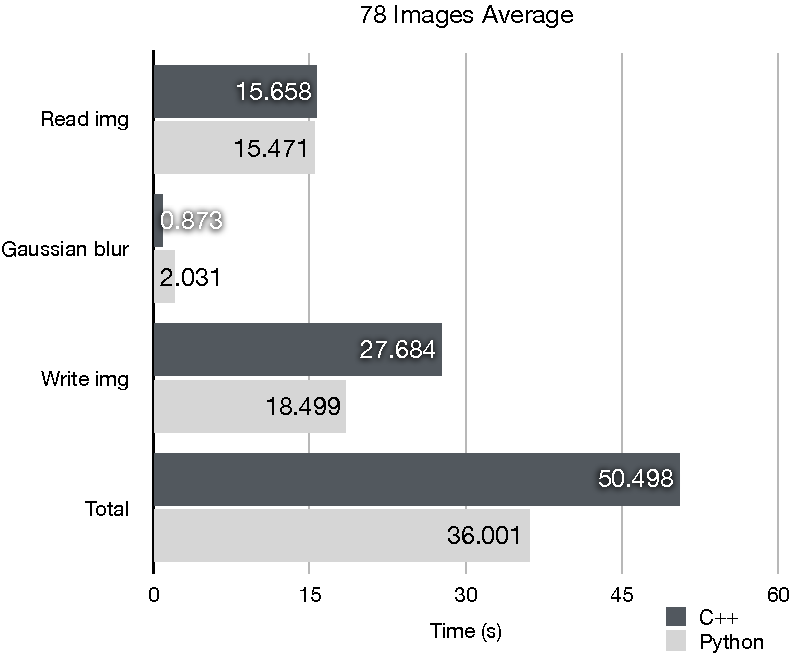
\includegraphics[width=1\linewidth]{average-without-script.pdf}
	  \caption{Average without script}
	  \label{fig:no-script}
	\end{subfigure}%
	\begin{subfigure}{.5\textwidth}
	  \centering
	  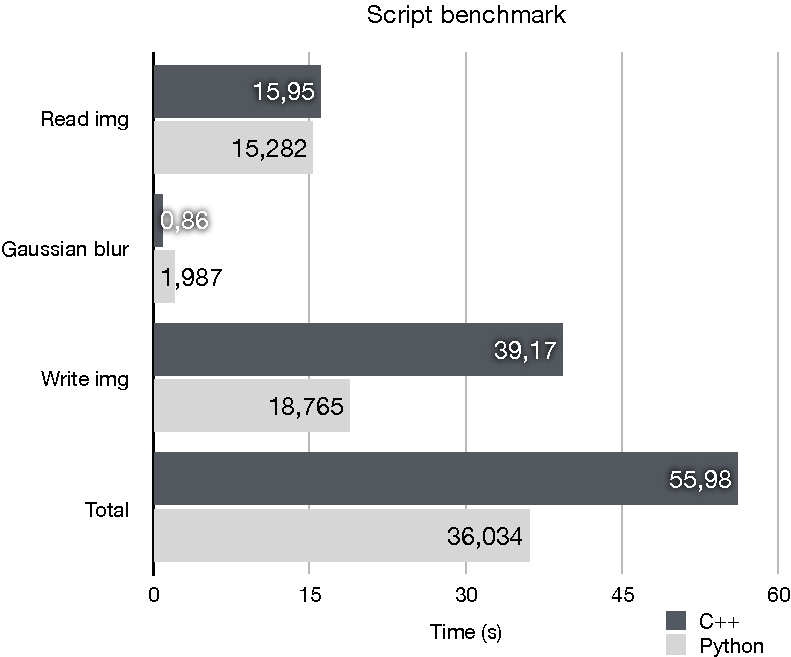
\includegraphics[width=1\linewidth]{script-benchmark.pdf}
	  \caption{Script benchmark}
	  \label{fig:script}
	\end{subfigure}
	\caption{Comparing the results of a script versus no script}
	\label{fig:script-vs-noscript}
\end{figure}

Figure 7.4 shows two benchmarks with a different script order, both using a RAMdisk. Each was measured by blurring 78 images. There is a slight difference between the two benchmarks, the randomised one running about two seconds faster. Overall, the proportions of the different benchmarks stayed the same.

\begin{figure}[H]
	\centering
	\begin{subfigure}{.5\textwidth}
	  \centering
	  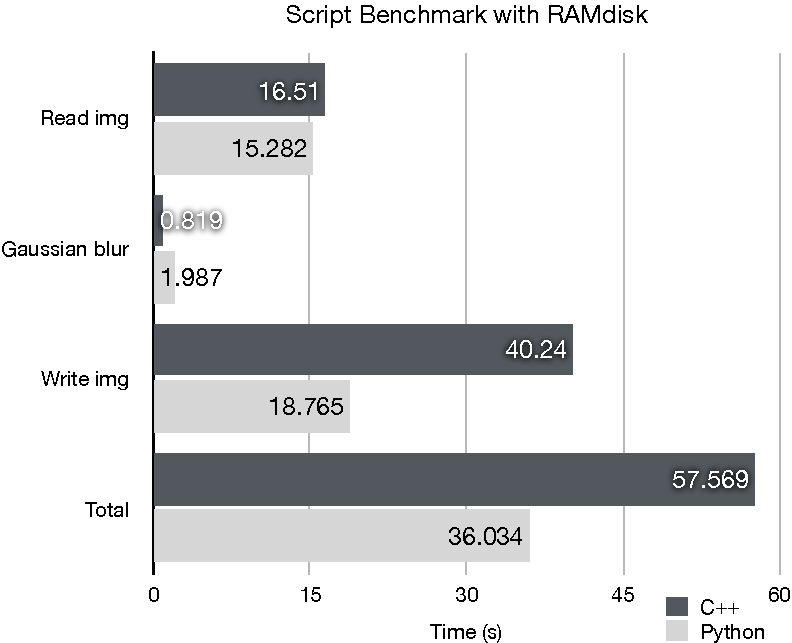
\includegraphics[width=1\linewidth]{ramdisk.pdf}
	  \caption{Script with RAMdisk}
	  \label{fig:ramdisk}
	\end{subfigure}%
	\begin{subfigure}{.5\textwidth}
	  \centering
	  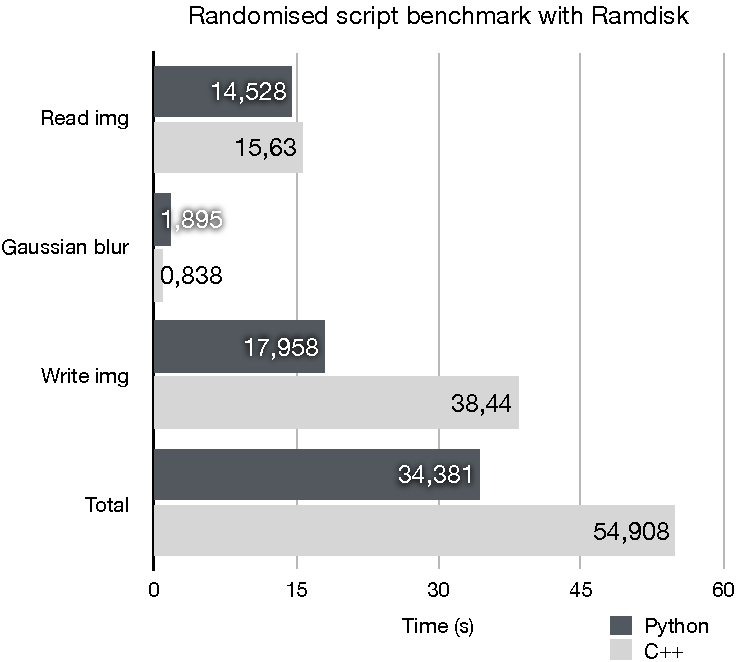
\includegraphics[width=1\linewidth]{random-ramdisk.pdf}
	  \caption{Randomised script with RAMdisk}
	  \label{fig:random-ramdisk}
	\end{subfigure}
	\caption{Comparing two different scripts}
	\label{fig:two-scripts}
\end{figure}

\section{RAMdisk}
A RAMdisk is a block of random-access memory that a computer's software is treating as if the memory were a disk drive. It can be used to accelerate the reading and writing of files. A RAMdisk was installed using the command "diskutil erasevolume HFS+ "RAMDisk" `hdiutil attach -nomount ram://2097152`" in the terminal. This creates a RAMdisk with 1 GB of storage space.
As seen in figure 7.5, compared to the benchmarks with no RAMdisk, running the scripted benchmarks with a RAMdisk surprisingly returns a decreased performance. However, the difference is so slight that we cannot confirm whether this is due to the RAMdisk or another influence.

\begin{figure}[H]
	\centering
	\begin{subfigure}{.5\textwidth}
	  \centering
	  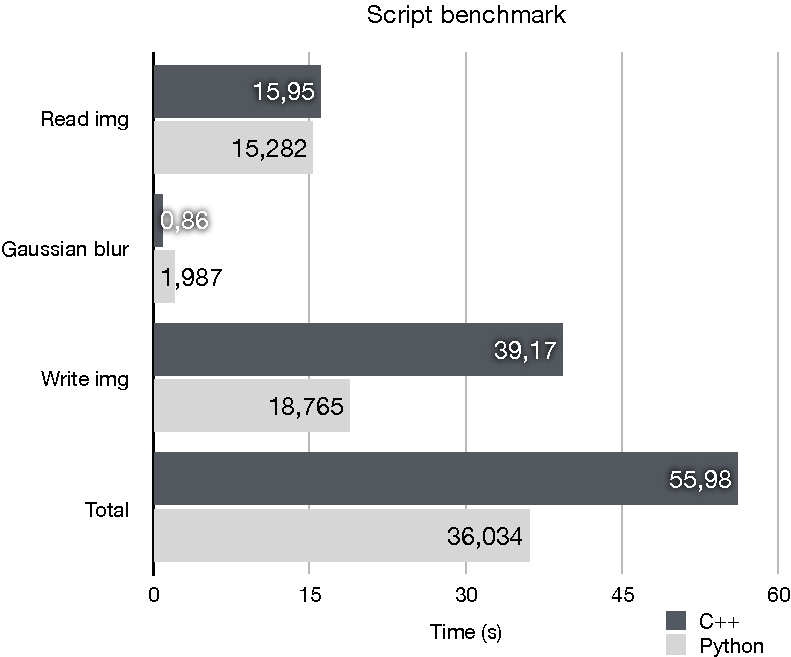
\includegraphics[width=1\linewidth]{script-benchmark.pdf}
	  \caption{Script without RAMdisk}
	  \label{fig:script2}
	\end{subfigure}%
	\begin{subfigure}{.5\textwidth}
	  \centering
	  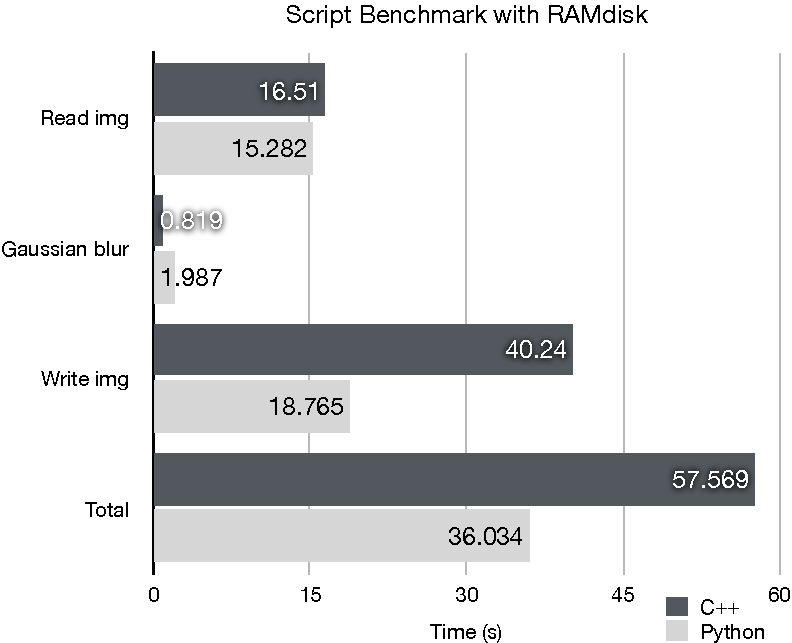
\includegraphics[width=1\linewidth]{ramdisk.pdf}
	  \caption{Script with RAMdisk}
	  \label{fig:ramdisk2}
	\end{subfigure}
	\caption{Comparing benchmarks with and without the use of a RAMdisk using the same script}
	\label{fig:ramdisk-vs-noramdisk}
\end{figure}

\section{Running the programs on a different computer}
In order to find out whether the computer hardware influenced the disk I/O, it was decided to test the programs on a different computer. The same computer type in a different configuration was utilised: the MacBook Pro from 2021 with an M1 Pro Apple Silicon CPU, 32 GB of RAM and a 1 TB SSD. To run the programs on this new configuration, it was needed to install Python version 3.10.3 instead of the previously used 3.8.12. The software was not compatible with the new M1 chip, so it had to be recompiled for Apple Silicon.
Figure 7.6 shows a similar distribution of runtime for the benchmark but an overall acceleration of 15 to 20 seconds compared to the other computer. The results are expected since this computer is a newer model and has more powerful hardware.

\begin{figure}[H]
	\centering
	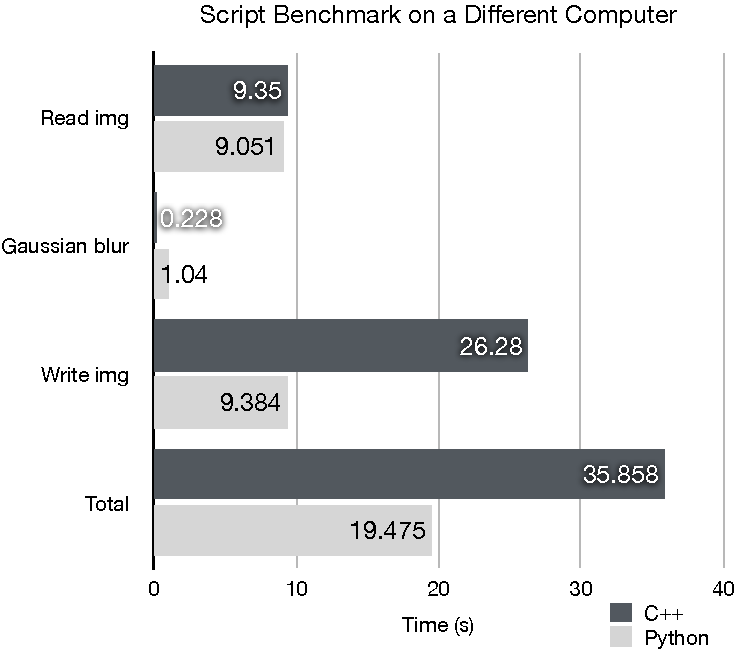
\includegraphics[scale=0.72]{different-comp.pdf}
	\caption{Script benchmark on a different computer}
	\label{figure:different-comp}
\end{figure}

\section{Profiling C++ and Python on Linux}
In order to rule out the possibility of the operating system influencing the unexpectedly slow C++ runtime, it was decided to experiment with our programs on a different operating system. An Ubuntu Linux instance was created using a virtual machine to benchmark the programs. This required some adjusting as the executable made for macOS was not compatible with Linux, and Linux obviously does not support the macOS instruments profiler. The C++ code was compiled with the cmake tool \cite{cmake} to create the new executable. The GCC (GNU Compiler Collection) \cite{gcc} compiler native fprofile command was used as a profiler. For Python, it was still possible to use the cProfile profiler. Each program was run five times and the average was calculated as seen in figure 7.7.
Interestingly, on Linux, the C++ program performed a lot faster than Python, 14.683 seconds faster, to be exact. This might once again be attributed to OpenCV being optimised differently for a different operating system and therefore performing better on Linux.

\begin{figure}[H]
	\centering
	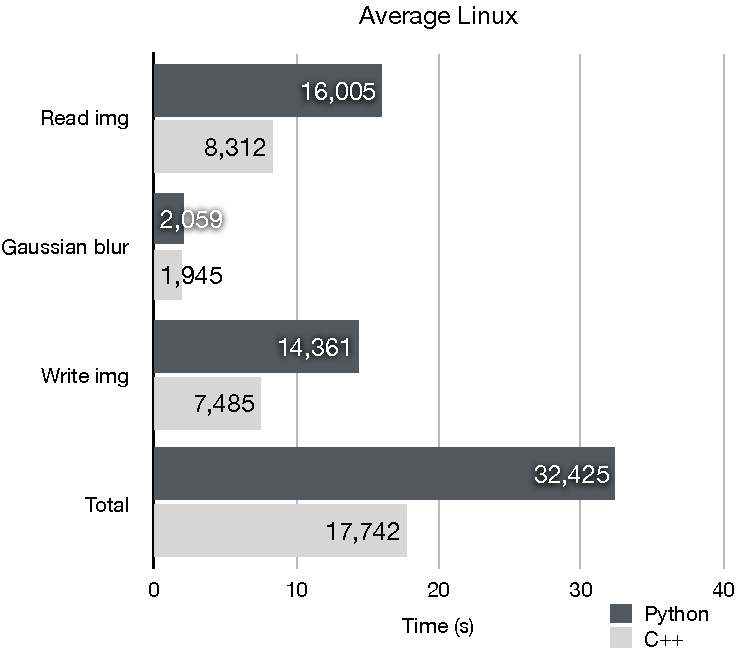
\includegraphics[scale=0.72]{linux.pdf}
	\caption{Average for the programs run on Linux}
	\label{figure:linux}
\end{figure}

\section{C++ using OpenCV from VCPKG}
One theory for the delay of C++ for disk output was that it was due to how the OpenCV library function handled writing to the disk. After doing further research, it was found that the standard OpenCV package for Python is a different version from what is standard for C++. Using VCPKG, a C/C++ dependency manager \cite{vcpkg}, the same version as used for Python was downloaded and used for C++. Benchmarking the programs with 100 randomly generated images shows the results in figure 7.9. Now, we can see only a very insignificant difference between the two programming languages compared to before.

\begin{figure}[H]
	\centering
	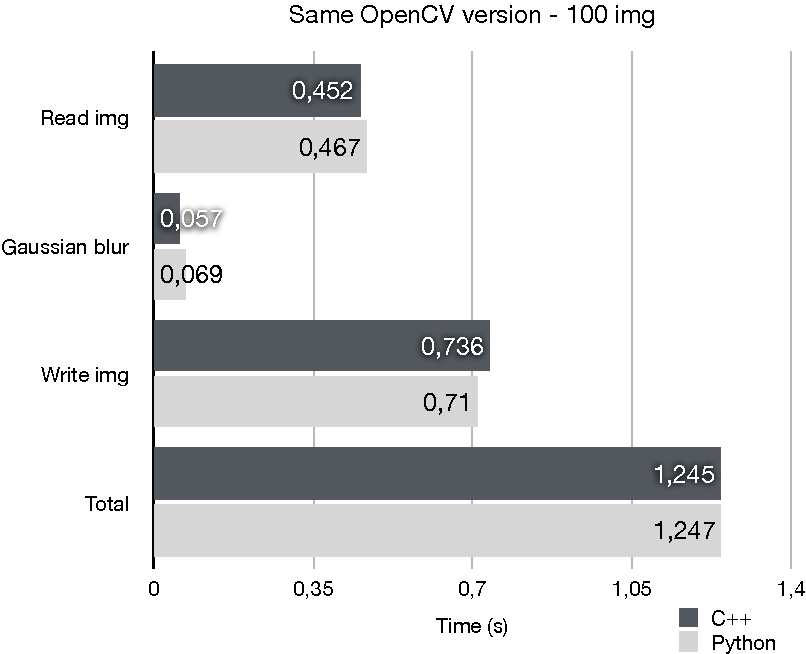
\includegraphics[scale=0.72]{same-opencv.pdf}
	\caption{Average of results using the same OpenCV version}
	\label{figure:same-opencv}
\end{figure}

We can see that the total runtime here is significantly less than when using the previous images. This can probably be attributed to the randomly generated images, which seem to have a lower resolution and are therefore faster to be processed. However, this is not important for this study as only the comparison of C++ and Python is of any consequence and not the overall performance.

\section{The error interval}
An error interval is a property of the instrument and the user and will remain the same for all readings taken, provided the scale is linear \cite{errorinterval}. It can be determined by finding the fraction of the smallest readable division on the instrument. In the case displayed in figure 7.9, benchmarking Python has yielded the error intervals in the last row, which is the same for each reading, using the same instrument.

\begin{figure}[H]
	\centering
	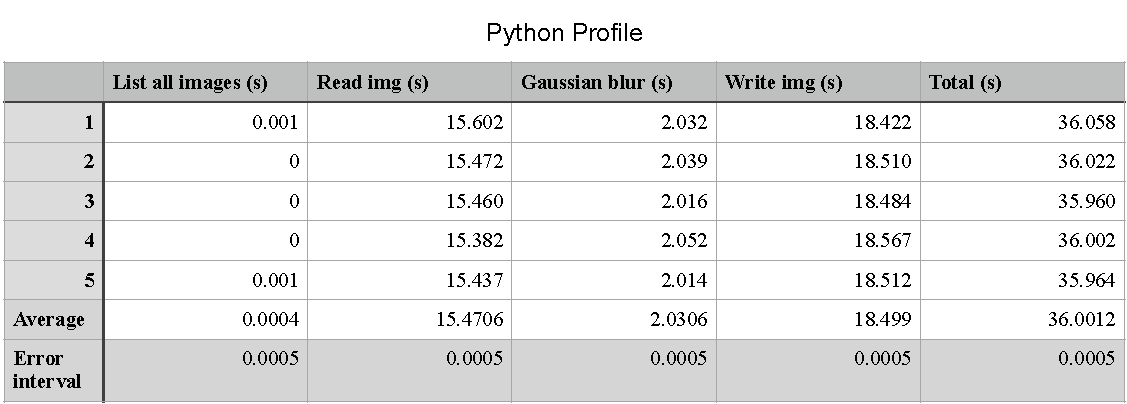
\includegraphics[scale=0.62]{error-interval.pdf}
	\caption{Python profiler average with error interval}
	\label{figure:error-interval}
\end{figure}

From this, we can determine that if we have a reading of, e.g. 18.500, with an error interval, it is actually between 18.4995 and 18.5005. Whilst this allows for a realistic interpretation of our measurements, it also does not affect any observations since all proportions are still the same.

\section{Energy consumption}
To confirm that runtime was congruous with energy consumption, the Intel Power Gadget was used to approximately measure the energy consumption of each program, both using the standard form of OpenCV with no RAMdisk. C++ had a runtime of 58.233 seconds in the experiment, and Python had a runtime of 38.889 seconds.
Figure 7.10 shows that the proportion of runtime to energy consumption is approximately the same. C++ used more energy than Python for the same program. Python’s runtime is 66.78\% of the C++ runtime, and Python’s energy consumption is 72.00\% of C++’s energy consumption overall and 72.30\% of the energy of the CPU/processor cores. These results indicate that runtime is an approximate indicator of energy consumption.

\begin{figure}[H]
	\centering
	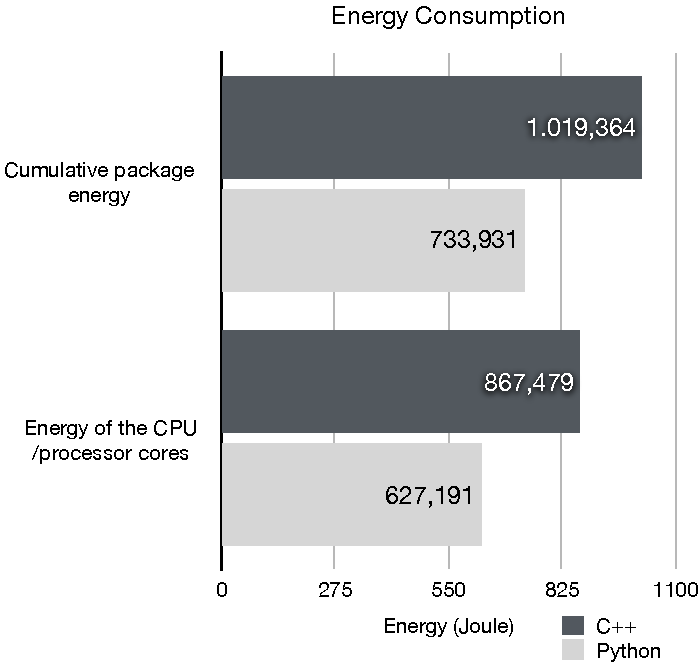
\includegraphics[scale=0.72]{energy.pdf}
	\caption{Energy consumption of the programs in Joule}
	\label{figure:energy-consumption}
\end{figure}

\chapter{Discussion}
Having experimented with many different configurations of the same program for both languages, we can make several observations. These observations are made only based on the image blurring programs for C++ and Python and cannot be generalised.
For one, we can say that on the MacBook Pros used for the experiments, Python performs faster by about 14 seconds than C++ for the standard OpenCV versions. Secondly, we can say that there is a difference in disk I/O for different image file types, which differ for the different languages. We also observed that using a script can provide more consistent data, and randomising said script can provide different results. Using a RAMdisk for disk I/O changes the total runtime, but the function runtimes' proportions stay the same. When running the programs on a different MacBook Pro, we observed a faster runtime overall but similar proportions yet again. Running the programs on a different operating system causes different results. On Linux, C++ ran approximately 14.7 seconds faster than Python. This is the direct opposite of running the programs on macOS. When running the scripted C++ program on macOS, we observed that we needed to change the version of the OpenCV library to measure similar results to the scripted Python program. Lastly, we primarily focus our research on measured proportions, so the error interval does not hold weight in this study.
These observations tell us that we cannot conclude from these experiments that the programming language itself makes a massive difference in optimisation. However, we can conclude that each minor change to the configuration of a program can make a big difference in the runtime and, therefore, the environmental impact.

\section{Influencing factors}
One part of the configuration of our program is the operating system. Operating systems control the computer’s hardware and manage software resources. There are many different types of operating systems, such as real-time, multitasking and embedded operating systems which all operate differently and therefore affect running a program differently.
Computers also have varying hardware. They can have a CPU, RAM or disk space of different sizes and speeds. They can also have different hardware altogether, such as having or not having an SSD (solid-state drive). For example, our standard MacBook Pro did not have an SSD, whilst the other MacBook Pro used for an experiment did have one, which made a difference in speed that might be attributed to that SSD.
We could also observe that different types of images might have influenced the runtime of the program. We used high-resolution space images for most experiments and we used automatically generated images for the experiment running OpenCV from VCPKG on C++, as seen in figure 8.1.

\begin{figure}[H]
	\centering
	\begin{subfigure}{.5\textwidth}
	  \centering
	  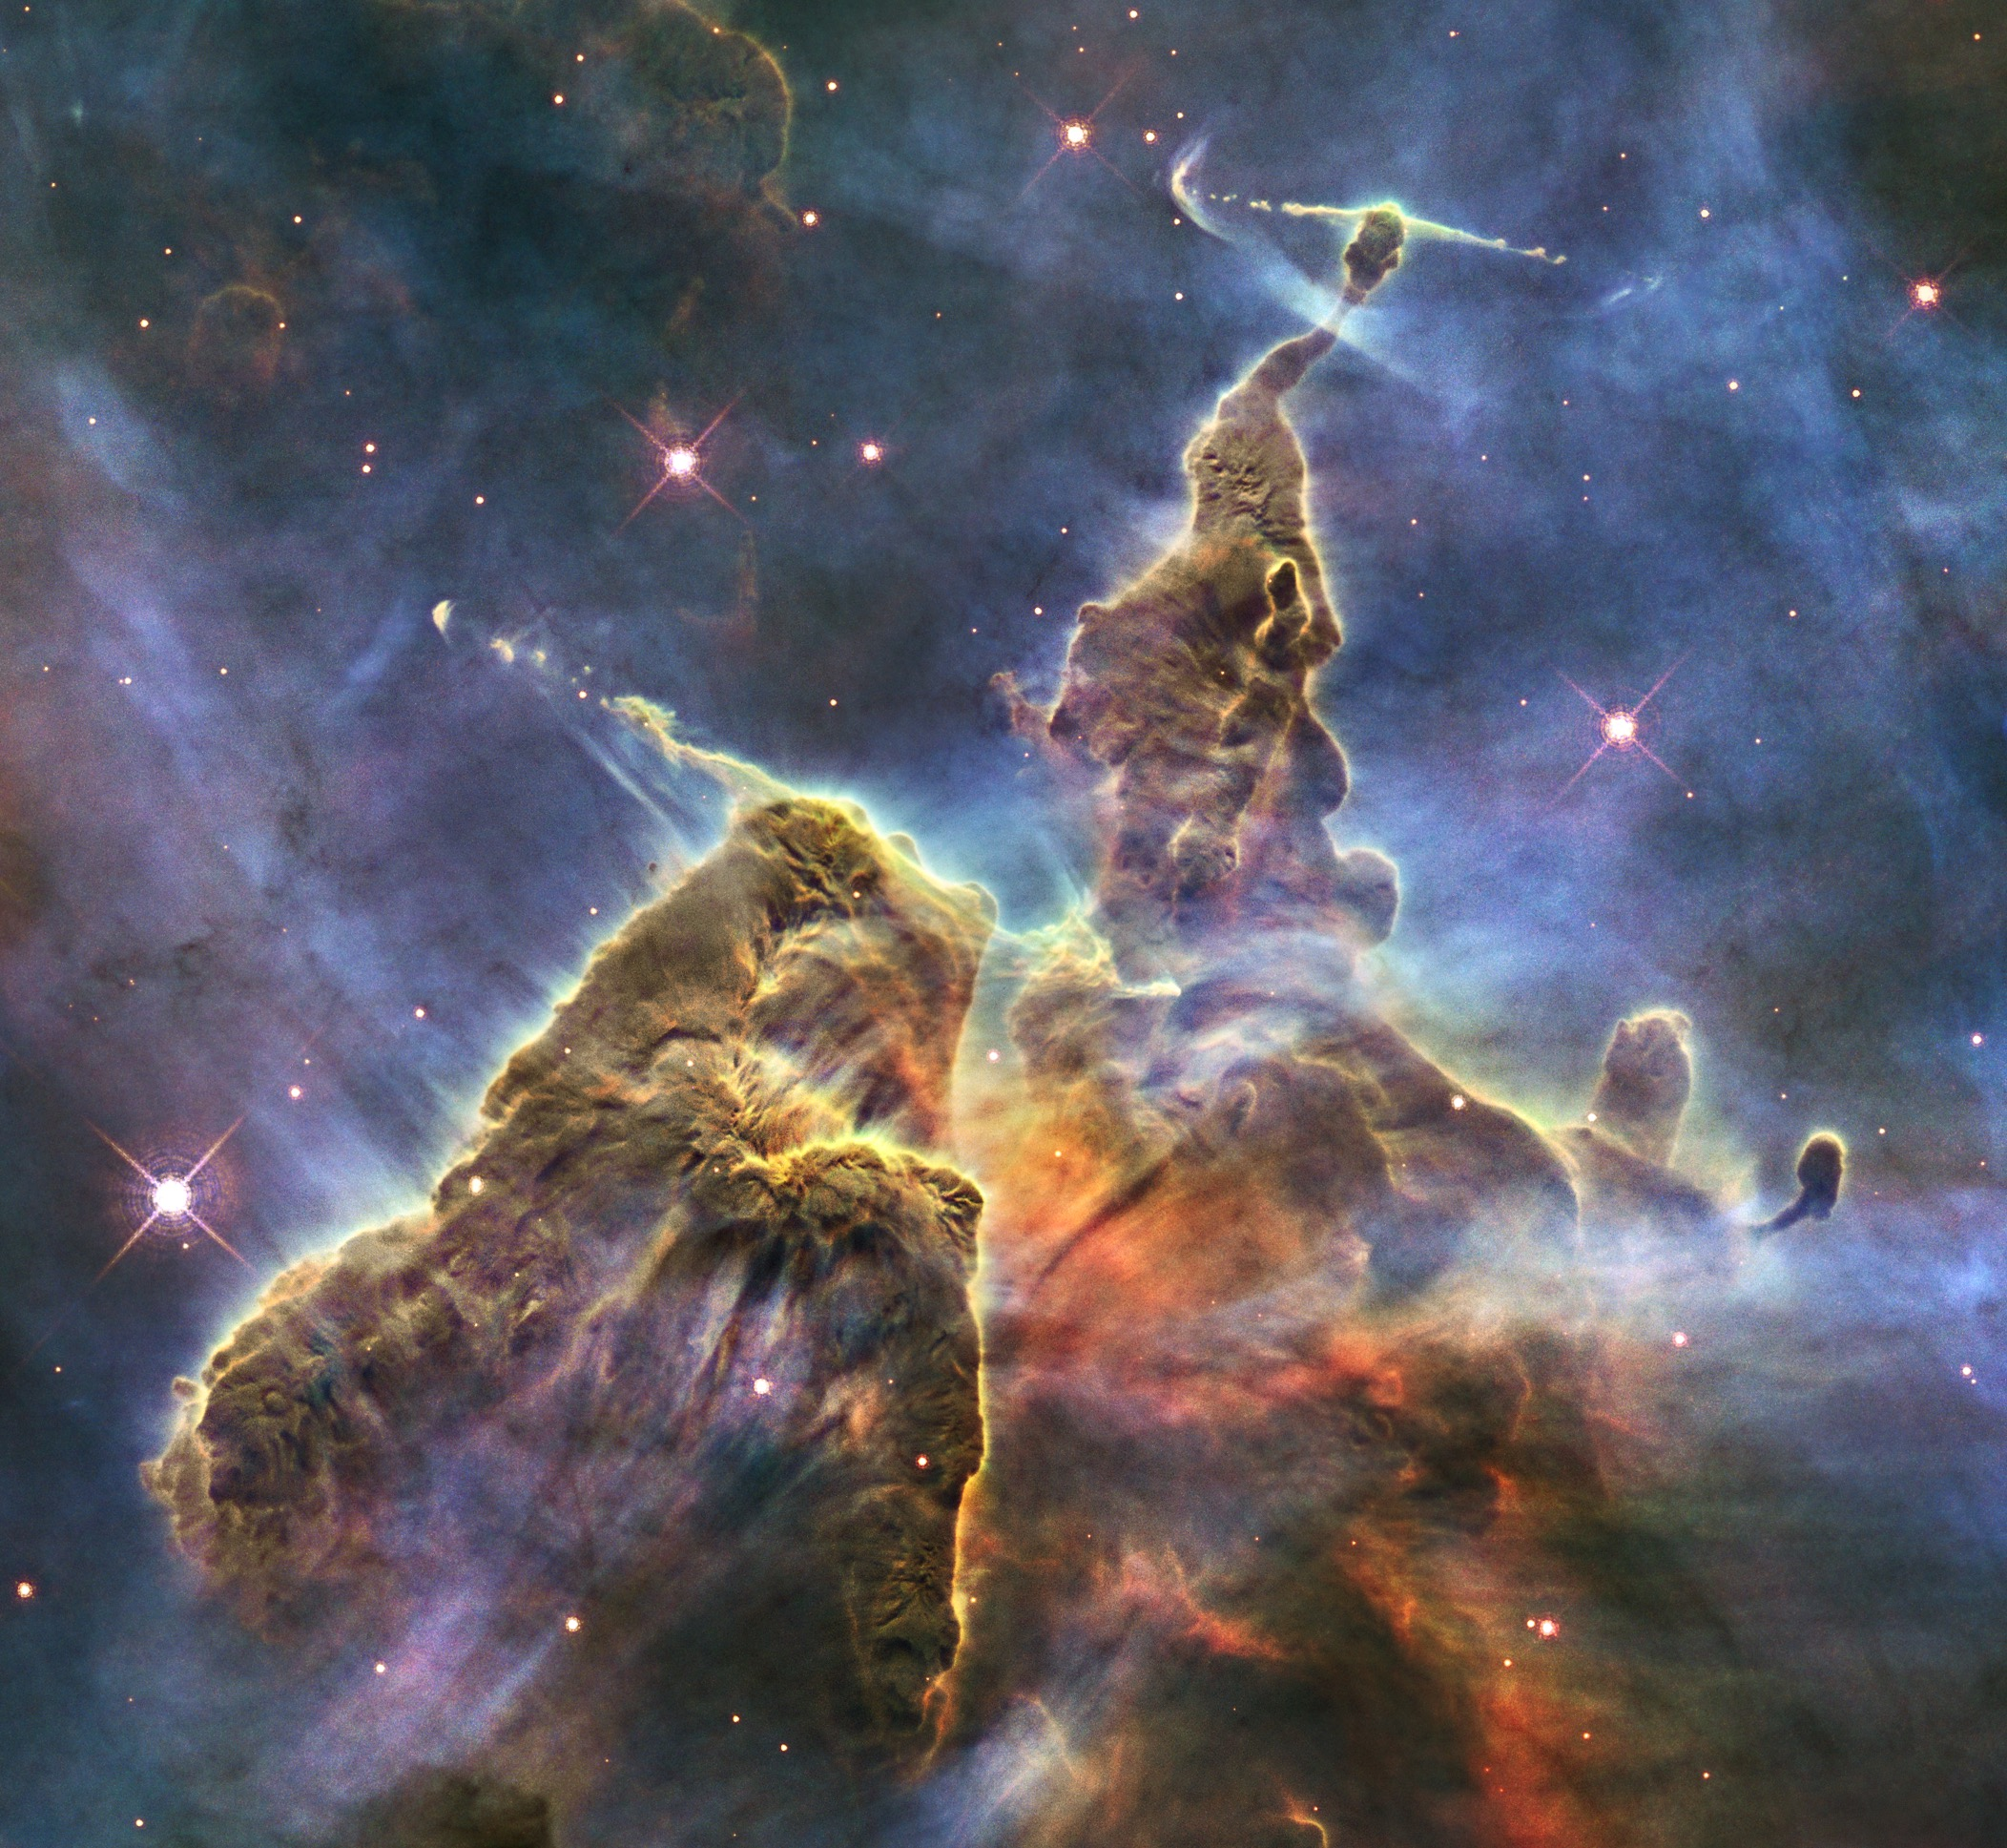
\includegraphics[width=1\linewidth]{high-res.jpeg}
	  \caption{High resolution image \cite{images}}
	  \label{fig:high-res-img}
	\end{subfigure}%
	\begin{subfigure}{.47\textwidth}
	  \centering
	  
\includegraphics[width=1\linewidth]{random-img.jpeg}
	  \caption{Randomly generated image}
	  \label{fig:random-img}
	\end{subfigure}
	\caption{a high-resolution image compared to a randomly generated image \cite{random_img}}
	\label{fig:test-images}
\end{figure}

We can see that image 8.1-a is a bit more complex than image 8.1-b, having colours and higher resolution. This means that blurring image 8.1-b might have been a bit faster than image 8.1-a, represented by the shorter runtime for the experiment running OpenCV from VCPKG on C++.
We observed a significant change in performance regarding different versions of a library. We also experimented with a different image processing library for Python called scikit-image \cite{scikit}. Scikit-image is written predominantly in Python. As seen in figure 8.2, scikit-image caused Python to perform significantly worse than C++ with OpenCV. Whereas when Python did use OpenCV, it performed better than C++. This proves to a certain extent that the type and version of a library are essential factors in optimisation.

\begin{figure}[H]
	\centering
	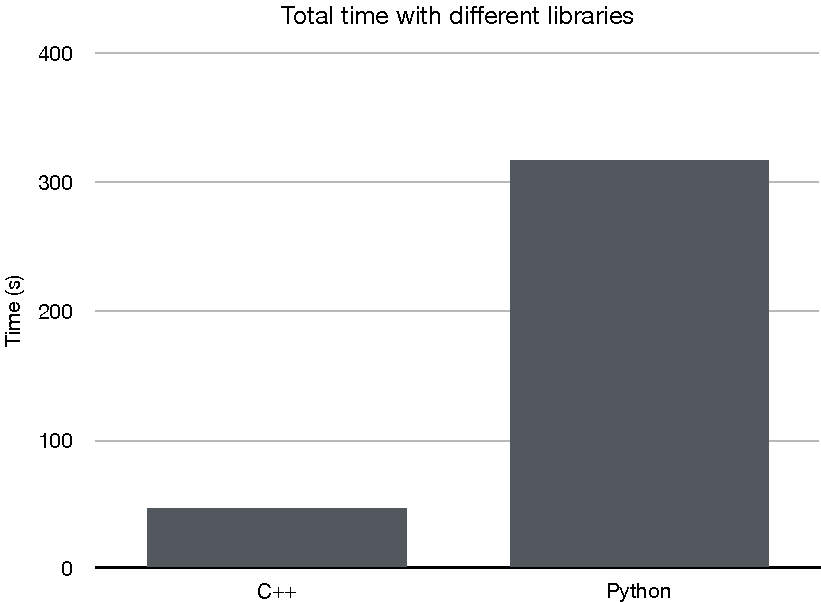
\includegraphics[scale=0.72]{scikit-total.pdf}
	\caption{Python total runtime using scikit-image to blur 79 images}
	\label{figure:scikit-total}
\end{figure}

Another factor that influences the runtime of a program is how the libraries are linked. The compilation of C++ involves three steps. First is preprocessing, which handles the preprocessor directives, such as “\#include” and “\#define” and, explained simply, replaces them with the content of the respective files. The next step is compilation, which takes the preprocessor’s output and produces an object file. The last step is linking. The linker takes the object files produced by the compiler and produces either a library or an executable file \cite{linking}. Linking can take two different forms. For one, static linking is the process of copying all library modules used in the program into the final executable image. Dynamic (or shared) linking adds the names of the libraries in the executable and then links them at runtime. Programs that use statically linked libraries are usually faster than those using shared libraries. When looking at the profile for C++, dyld was shown as taking up a lot of the total runtime. Dyld is a macOS pre-linking of dynamic libraries. Chandler Caruth, a principal software developer at Google, mused in a Twitter feed about the general slow runtime of a program on macOS as compared to Linux and found that it was due to spending a vast amount of time on dyld \cite{twitter}. This matches what we observed with the xctrace profiler CPU counter.
Of course, the programming language also plays a role in program optimisation. We already saw from previous research that the programming language can influence the runtime for a specific algorithm. Lack of knowledge of the language can cause it to be written in a way that delays the runtime. Additionally, in real-life programming, programmers hardly ever write the entirety program themselves; they use external libraries, packages or models. Choosing the wrong library for our configuration can lead to significant delays, as we have proved in this study. Therefore, choosing a language for a project might be based on available libraries but should also be chosen on the characteristics of the language and if they are optimised for the project. In conclusion, we can say that every program needs its own particular configuration of hardware, OS, language, compilation, external libraries and whichever other factors might contribute.

\chapter{Conclusion}
This research aimed to identify the environmental impact of the choice of programming language. Based on a series of experiments, we can conclude that the choice of programming language can only impact the runtime if all other factors of the program's configuration are optimised.
We benchmarked the same program in two different languages and in a multitude of different configurations to find which impact the language would make. We expected to see C++ perform better than Python for the image processing program. The results did not match our expectations, and experiments were done to explain these results. These experiments resulted in the observation that minor differences in the configuration of a program can make a big difference in total runtime.
A limitation of the research is the scale. Provided with more time and resources, it would have been interesting to experiment with the program on more operating systems, different hardware, and more library variations. Additionally, to better understand the pure impact of the programming language, it would have been interesting to forgo libraries altogether and write all functionality from scratch to receive ultimate control over the program. Another approach could be to experiment with more programming languages to find the nuances that set them apart for different purposes.
This research contributes the knowledge that when we want to make an environmental impact with our software, we need to optimise every part of the configuration of a program, including choosing the best programming language for the purpose.


% \clearpage
% \phantomsection
% \addcontentsline{toc}{chapter}{Bibliography}
% \setlength{\bibitemsep}{10pt}
% \renewcommand{\baselinestretch}{1.1}
% \sloppy
% \printbibliography

\bibliographystyle{plain}
\bibliography{./references.bib}

\clearpage
\phantomsection
\addcontentsline{toc}{chapter}{Affidavit}

\chapter*{Affidavit}
I hereby confirm that I have written the thesis titled "\thetitle" by myself, without contributions from any sources other than those cited in the text and bibliography. This also applies to all graphics, drawings, and images included in the thesis.

Furthermore, I confirm that neither this work nor parts of it have been previously or concurrently used as an assessment submission in other courses or in other examination proceedings.

Berlin, 07.06.2022,




\end{document}

